%
% REWRITING OPEN OBJECTS
% Open objects in a topos
% v1
%

% --- comment out when compiling ---
%
%	REWRITING OPEN GRAPHS
%	preamble
%	v1

%  packages

\usepackage{amsfonts, amsthm, amssymb, amsmath, stmaryrd, etoolbox}
\usepackage{mathtools}
\usepackage{graphicx,caption,subcaption}
\usepackage{todonotes}
\usepackage{xcolor}
\usepackage{url}
\usepackage[inline]{enumitem}
	\setlist{itemsep=0em, topsep=0em, parsep=0em}
	\setlist[enumerate]{label=(\alph*)}
\usepackage[]{hyperref}
	\definecolor{hyperrefcolor}{rgb}{0,0,0.7}
	\hypersetup{colorlinks,linkcolor={hyperrefcolor},citecolor={hyperrefcolor},urlcolor={hyperrefcolor}}
\usepackage{tikz}
	\usetikzlibrary{matrix,arrows,shapes,decorations.markings,decorations.pathreplacing}
\usepackage[numbers]{natbib}
\usepackage{doi}

%
% commands
%

\newcommand{\RR}{\mathbb{R}}
\newcommand{\ZZ}{\mathbb{Z}}
\newcommand{\NN}{\mathbb{N}}
\newcommand{\QQ}{\mathbb{Q}}
\newcommand{\CC}{\mathbb{C}}
\newcommand{\DD}{\mathbb{D}}
\newcommand{\MM}{\mathbb{M}}
\renewcommand{\epsilon}{\varepsilon}

\newcommand{\defn}[1]{\textbf{#1}}
\newcommand{\op}[1]{\operatorname{#1}}
\newcommand{\cat}[1]{\mathbf{#1}}
\newcommand{\dblcat}[1]{\mathbb{#1}}
\renewcommand{\t}[1]{\text{#1}}

\newcommand{\from}{\colon}
\newcommand{\xto}[1]{\xrightarrow{#1}}
\newcommand{\sm}{\smallsetminus}
\newcommand{\tospan}{\xrightarrow{\mathit{sp}}}
\newcommand{\tocospan}{\xrightarrow{\mathit{csp}}}
\newcommand{\diagram}[1]{\raisebox{-0.5\height}{\includegraphics{#1}}}

\newcommand{\bispmap}[1]{\mathbf{Sp(#1)}}
\newcommand{\dblspmap}[1]{\mathbb{S}\mathbf{p(#1)}}
\newcommand{\bicspmap}[1]{\mathbf{Csp(#1)}}
\newcommand{\dblcspmap}[1]{\mathbb{C}\mathbf{sp(#1)}}
\newcommand{\bispsp}[1]{\mathbf{Sp(Sp(#1))}}
\newcommand{\dblspsp}[1]{\mathbb{S}\mathbf{p(Sp(#1))}}
\newcommand{\bicspcsp}[1]{\mathbf{Csp(Csp(#1))}}
\newcommand{\dblcspcsp}[1]{\mathbb{C}\mathbf{sp(Csp(#1))}}
\newcommand{\bimonspcsp}[1]{\mathbf{MonicSp(Csp(#1))}}
\newcommand{\dblmonspcsp}[1]{\mathbb{M}\mathbf{onicSp(Csp(#1))}}
\newcommand{\biepiccspsp}[1]{\mathbf{EpicCsp(Sp(#1))}}
\newcommand{\dblepiccspsp}[1]{\mathbb{E}\mathbf{picCsp(Sp(#1))}}
\newcommand{\spcsp}[1]{\mathbf{Sp(Csp(#1))}}
\newcommand{\dblspcsp}[1]{\mathbb{S}\mathbf{p(Csp(#1))}}

\newcommand{\LspanD}{ L \t{-} \operatorname{Span} ( \mathbf{D} ) }
\newcommand{\LopenD}{ L \t{-} \operatorname{Open} }
\newcommand{\LrewriteD}{ L \t{-} \operatorname{Rewrite} }

%
% math operators
%

\DeclareMathOperator{\Hom}{Hom}
\DeclareMathOperator{\id}{id}
\DeclareMathOperator{\ob}{Ob}
\DeclareMathOperator{\arr}{arr}
\DeclareMathOperator{\im}{im}
\DeclareMathOperator{\Aut}{Aut}
\DeclareMathOperator{\Bij}{Bij}
\DeclareMathOperator{\Sub}{Sub}
\DeclareMathOperator{\colim}{colim}

%
% envirnments and counters
%

\newtheorem{thm}{Theorem}[section]
\newtheorem{lem}[thm]{Lemma}
\newtheorem{prop}[thm]{Proposition}
\newtheorem{cor}[thm]{Corollary}

\theoremstyle{remark}
	\newtheorem{remark}[thm]{Remark}
	\newtheorem{notation}[thm]{Notation}

\theoremstyle{definition}
	\newtheorem{ex}[thm]{Example} 
	\newtheorem{df}[thm]{Definition}

% \setcounter{tocdepth}{1} % Sets depth for table of contents. 

%
% tikz types
%

\tikzset{->-/.style={decoration={%
			markings,
			mark=at position .5 with {\arrow{>}}},postaction={decorate}}
}
\tikzset{->-pos/.style={decoration={%
			markings,
			mark=at position #1 with {\arrow{>}}},postaction={decorate}}
}
\tikzset{->-/.style={decoration={%
			markings,
			mark=at position .5 with {\arrow{>}}},postaction={decorate}}
}
\tikzset{->-pos/.style={decoration={%
			markings,
			mark=at position #1 with {\arrow{>}}},postaction={decorate}}
}
 
\bibliography{3--RewriteOpenGraphs--Bibliography} 

\section{Open objects in a topos} 

In this section, we consider
the notion of an `open object'. 
We start with a brief discussion of open graphs to help us develop an intuition. 
As we will see,
an open object is a certain
cospan. However, the context in which
we plan to use open objects is
novel enough to warrant this introduction.
Since our motivation is to use open objects
to study network theory, which makes
heavy use of various sorts of graphs,
we focus our attention to open objects 
\emph{in a topos} and show that these 
form a topos themselves. 

% open graphs------------

\subsection*{Open Graphs}

Conceptually, open graphs 
are quite simple.  
Take a directed graph 
and declare some of the nodes 
to be inputs and 
others to be outputs, 
for example
\begin{equation}
\label{ex--OpenGraph1}
\raisebox{-0.5\height}{
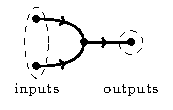
\includegraphics{InclGrphx--Example--OpenGraph1}
}
\end{equation}

Given open graphs $G$ and $G'$,
if the set of inputs in $G$
and the set of outputs in $G'$
have the same cardinality,
we can glue them together
along a bijection.
This gives a way 
to turn a pair of 
compatible open graphs
into a single open graph.  
For instance, 
to the above open graph, 
we can connect 
\begin{equation}
\label{ex--OpenGraph2}
\raisebox{-0.5\height}{
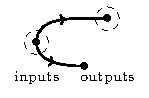
\includegraphics{InclGrphx--Example--OpenGraph2}
}
\end{equation}
to form
\begin{equation}
\label{ex--OpenGraph3}
\raisebox{-0.5\height}{
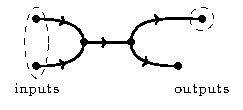
\includegraphics{InclGrphx--Example--OpenGraph3}
}
\end{equation}
We make this precise with
cospans and pushouts.

\todo{
	past considerations of open graphs
}

Consider the functor
\begin{equation}
\label{eq--FunctorN}
	N \colon \mathbf{FinSet} \to \mathbf{FinGraph},
\end{equation}
defined by the letting 
$N(x)$ be the edgeless graph 
with nodes $x$.  

\begin{df} % open graphs
	\label{df--OpenGraph}
	An \emph{open graph} is then 
	a cospan in the category 
	$\mathbf{FinGraph}$ 
	of the form 
	$N(x) \to g \gets N(y)$ 
	for sets $x$ and $y$.
	Given another open graph
	$N(x') \to g' \gets N(y')$, 
	a morphism between them
	is a triple $(f,g,h)$ so that
	the diagram
	\[
	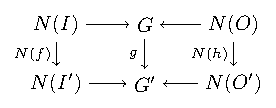
\includegraphics{InclGrphx--Diagram--OpenGraphMap}
	\]
	commutes.
	Open graphs and their morphisms
	form a category $\cat{OpenGraph}$.	
\end{df}

How does a cospan outfit a graph
with inputs and outputs?
The left leg $N(x)$ of the cospan 
selects the \emph{inputs} and 
the right leg $N(y)$ the \emph{outputs}.  
We will refer to the union
of the inputs and outputs as the
\emph{boundary} of an open graph.
The addition of a boundary allows us to 
`glue' certain open graphs together
to produce another open graph.
Indeed, suppose we have open graphs 
\[
	N ( X ) \to G \gets N ( Y )
	\t{ and }
	N ( Y ) \to H \gets N ( Z ).
\]
Then we can concatenate the cospans 
\[
	N(X) \to G \gets N(Y) \to H \gets N(Z). 
\] 
and obtain another open graph
by pushing out over 
$G \gets N(Y) \to G'$ to get 
\[
	N(X) \to G +_{ N ( Y ) } H \gets N(Z).
\] 

To illustrate this, 
realize the open graph in \eqref{ex--OpenGraph1}
as the cospan of graphs
\begin{equation}
\label{ex--OpenGraphCospan1}
	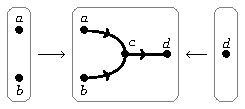
\includegraphics{InclGrphx--Example--OpenGraphCospan1}
\end{equation}
Similarly, we realize \eqref{ex--OpenGraph2} as 
\[
	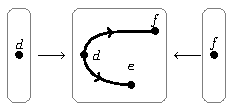
\includegraphics{InclGrphx--Example--OpenGraphCospan2}
\]
Now, pushout over
the middle span in the concatenated
cospans
\[
	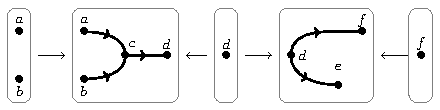
\includegraphics{InclGrphx--Example--OpenGraphCospan3}
\]
The result is
\[
	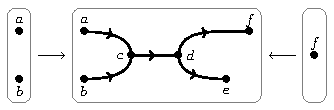
\includegraphics{InclGrphx--Example--OpenGraphCospan4}
\]
which realizes 
\eqref{ex--OpenGraph3} 
as a cospan.

% open objects in topoi

At its core, constructing open graphs
does not rely on combinatorial properties
of graphs, but rather on categorical properties.  
This is good news, because our interests
lie in working with many different sorts of graphs. 
Therefore, we give a general construction
of \emph{categories of open objects}.  
One might be tempted to define such a thing
as $\cat{C}$-valued pres-sheaves on 
the walking cospan, for $\cat{C}$ having pushouts.
However, our considerations require that
we can develop a decent theory of rewriting
for our \emph{open objects}. 
In particular, we ask that whatever 
we define open objects to be, that they form
an adhesive category.  To this end,
we restrain ourselves from taking
the above naive approach and, instead,
tread a bit more carefully. 

We begin our construction with an
adjoint pair between topoi
\[
	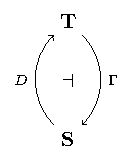
\includegraphics{InclGrphx--Diagram--AdjointPair}
\]
We denote the right adjoint by $\Gamma$
and the left adjoint by $D$ as they
will behave similar to the global sections
and discrete functors, respectively,
found in cohesive topos theory.
Using this adjoint pair, we
present the following definition.

\begin{df}
	An \defn{$\cat{S}$-open object in $\cat{T}$} is 
	a cospan in $\cat{T}$ of form 
	\[
		D ( x ) \to t \gets D ( y ) .
	\]
	Morphisms are triples $(f,g,h)$ 
	that fit into a commuting diagram
	\[
		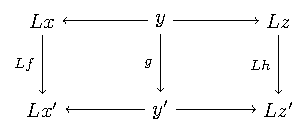
\includegraphics{InclGrphx--Diagram--OpenObjectArrow}
	\]
	This forms a category $\cat{S\t{-}OpenObj}(\cat{T})$.	
\end{df}

\begin{thm}
	The category $\cat{S\t{-}OpenObj}(\cat{T})$
	is a topos.
\end{thm}
\begin{proof}
	By adjointness, $\cat{S\t{-}OpenObj}(\cat{T})$
	is equivalent to the category with
	cospans of form 
	\[
		x \to \Gamma (t) \gets y
	\]
	and triples $(f,g,h)$ fitting into
	the commuting diagram
	\[
		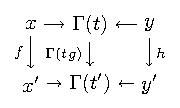
\includegraphics{InclGrphx--Diagram--OpenObjectAdjointArrow}
	\]	
	But this is equivalent to the 
	comma category $(S \times S) / \Delta \Gamma$,
	for $\Delta \from S \to S \times S$ the diagonal functor.
	But $\Delta \Gamma$ preserves finite limits which,
	by a result of Wraith \cite{Wraith_ArtinGlue}, implies
	that $(S \times S) / \Delta \Gamma$ is a topos.	
\end{proof}

\todo{dble check those equivalences}

Open graphs fit nicely into this framework.
Consider the adjoint pair
\[
	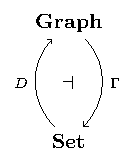
\includegraphics{InclGrphx--Diagram--AdjointPairOpenGraphs}
\]
where $\Gamma$ is the underlying node functor
and $D$ sends a set to the corresponding
discrete graph.  
  